% Math and Comp Sci Student
% Homework template by Joel Faubert
% Ottawa University
% Fall 2018
%
% This template uses packages fancyhdr, multicol, esvect and amsmath
% http://ctan.cms.math.ca/tex-archive/macros/latex/contrib/esvect/esvect.pdf
% http://www.ams.org/publications/authors/tex/amslatex
%
% These packages are freely distribxted for use but not
% modification under the LaTeX Project Public License
% http://www.latex-project.org/lppl.txt

\documentclass[letterpaper, 10pt]{article}
% \usepackage[text={8in,10in},centering, margin=1in,headheight=28pt]{geometry}
\usepackage[margin=1in, centering, headheight=28pt]{geometry}
\usepackage{fancyhdr}
\usepackage{esvect}
\usepackage{amsmath}
\usepackage{bbold}
\usepackage{amsfonts}
\usepackage{amssymb}
\usepackage{amsthm}
\usepackage{mathrsfs}
\usepackage{mathtools}
\usepackage{multicol}
\usepackage{enumitem}
\usepackage{verbatimbox}
\usepackage{fancyvrb}
\usepackage{hyperref}
\usepackage[pdftex]{graphicx}
\graphicspath{ {./results/} }
\usepackage[space]{grffile}
\usepackage{tikz}
\usetikzlibrary{arrows.meta}
\usetikzlibrary{positioning}
\usepackage{bm}
\usepackage{minted}
\usepackage{longtable}
\usepackage{caption}
\captionsetup{skip=10pt}

\pagestyle{fancy}
\paperwidth 8.5in
\paperheight 11in

% Configxre headers and footers

\lhead{CSI5138 \\ Prof. Yongyi Mao }
\rhead{Jo\"el Faubert \\ Student \# 2560106}
\chead{Assignment 4 \\ 25-11-2018}
\rfoot{\today}
\fancyhfoffset[l]{40pt}
\fancyhfoffset[r]{40pt}
\renewcommand{\headrulewidth}{0.4pt}
\renewcommand{\footrulewidth}{0.4pt}
\setlength{\parskip}{10pt}
\setlist[enumerate]{parsep=10pt, itemsep=10pt}

% Define shortcuts

\newcommand{\floor}[1]{\lfloor #1 \rfloor}
\newcommand{\ceil}[1]{\lceil #1 \rcleil}

% matrices
\newcommand{\bpm}{\begin{bmatrix}}
\newcommand{\epm}{\end{bmatrix}}
\newcommand{\vm}[3]{\begin{bmatrix}#1\\#2\\#3\end{bmatrix}}
\newcommand{\Dmnt}[9]{\begin{vmatrix}#1 & #2 & #3 \\ #4 & #5 & #6 \\ #7 & #8 & #9 \end{vmatrix}}
\newcommand{\dmnt}[4]{\begin{vmatrix}#1 & #2 \\ #3 & #4 \end{vmatrix}}
\newcommand{\mat}[4]{\begin{bmatrix}#1 & #2\\#3 & #4\end{bmatrix}}

% common sets
\newcommand{\R}{\mathbb{R}}
\newcommand{\Qu}{\mathbb{Q}}
\newcommand{\Na}{\mathbb{N}}
\newcommand{\Z}{\mathbb{Z}}
\newcommand{\Rel}{\mathcal{R}}
\newcommand{\F}{\mathcal{F}}
\newcommand{\U}{\mathcal{U}}
\newcommand{\V}{\mathcal{V}}
\newcommand{\K}{\mathcal{K}}
\newcommand{\M}{\mathcal{M}}

% Power set
\newcommand{\PU}{\mathcal{P}(\mathcal{U})}

%norm shortcut
\DeclarePairedDelimiter{\norm}{\lVert}{\rVert}

% projection, vectors
\DeclareMathOperator{\proj}{Proj}
\newcommand{\vctproj}[2][]{\proj_{\vv{#1}}\vv{#2}}
\newcommand{\dotprod}[2]{\vv{#1}\cdot\vv{#2}}
\newcommand{\uvec}[1]{\boldsymbol{\hat{\textbf{#1}}}}

% derivative
\def\D{\mathrm{d}}

% big O
\newcommand{\bigO}{\mathcal{O}}

% probability
\newcommand{\Expected}{\mathrm{E}}
\newcommand{\Var}{\mathrm{Var}}
\newcommand{\Cov}{\mathrm{Cov}}
\newcommand{\Entropy}{\mathrm{H}}
\newcommand{\KL}{\mathrm{KL}}

\DeclareMathOperator*{\argmax}{arg\,max}
\DeclareMathOperator*{\argmin}{arg\,min}

\setlist[enumerate]{itemsep=10pt, partopsep=5pt, parsep=10pt}
\setlist[itemize]{itemsep=5pt, partopsep=5pt, parsep=10pt}

\begin{document}
\section{Introduction and Acknowledgements}

This report compares the results of three density estimation algorithms:
Variational Autoencoders (VAE), Generative Adversarial Networks (GAN) and Wasserstein-GANs (WGAN).

Models are built using the MNIST and CIFAR10 data sets.

As a preprocessing step, the words images are converted to tensors and normalized.

A module for loading the data ({\em load\_data.py}) encapsulates the DataLoader functions of PyTorch.
Thankfully, loaders for both of these datasets are available in the Torchvision package.

The VAE code is based on \url{https://github.com/pytorch/examples/blob/master/vae/main.py}

The GAN code is based on \url{https://pytorch.org/tutorials/beginner/dcgan_faces_tutorial.html}

Finally, the WGAN is based on \url{https://wiseodd.github.io/techblog/2017/02/04/wasserstein-gan/}

For each of these algorithms, I contrast generated images with real sample images and examine the plot of the loss functions during training.

\section{Variational Autoencoder}

For this first VAE model ({\em vae.py}), the model is a simple fully-connected hourglass-structure with a bottleneck of dimension 20.

\begin{figure}[h]
\caption{MNIST VAE Reconstructions After 20 Training Epochs}
\centering
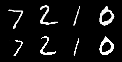
\includegraphics[width=0.75\textwidth]{vae_reconstruction_20_epochs}
\end{figure}

\begin{figure}[h]
\caption{CIFAR10 VAE Reconstructions After 20 Training Epochs}
\centering
\includegraphics[width=0.75\textwidth]{cifar10_reconstruction_20_epochs}
\end{figure}

\section{Generative Adversarial Network}

GANs were first described in \cite{goodfellow2014generative}. 
In my first attempt, I used modeled the generator and discriminator networks using fully-connected layers but the results were unimpressive.

For my second attempt, I followed the tutorial linked above which is based on \cite{radford2015unsupervised},
in which the authors implement the discriminator and generator using convolutions (and so-called transpose convolutions).
Below are sample images generated after 25 and 50 training epochs.

\begin{figure}[h]
\caption{DCGAN Generated MNIST Images After 50 Epochs}
\centering
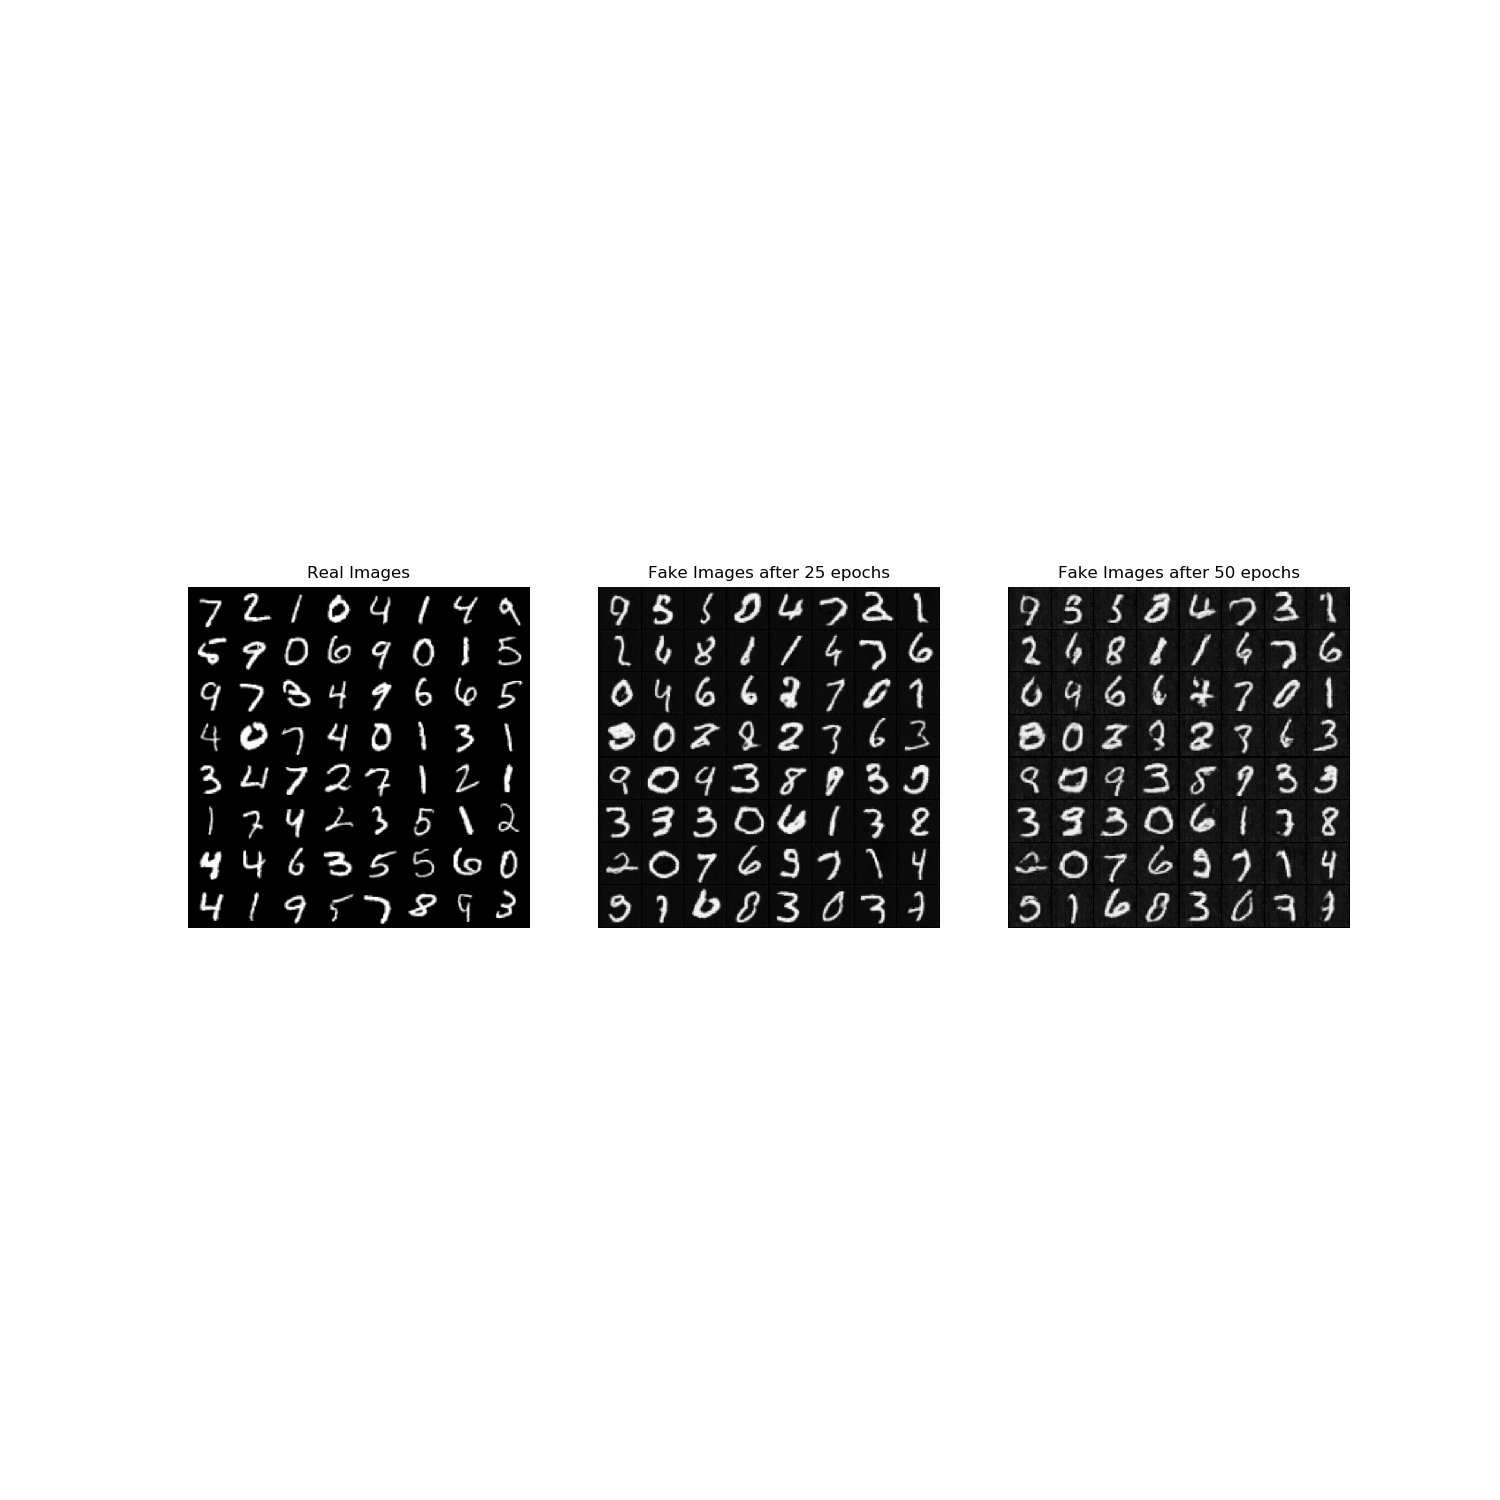
\includegraphics[width=0.75\textwidth]{mnist_gan_real_v_fake_50_epochs}
\end{figure}

\begin{figure}[h]
\caption{DCGAN Generated CIFAR10 Images After 50 Epochs}
\centering
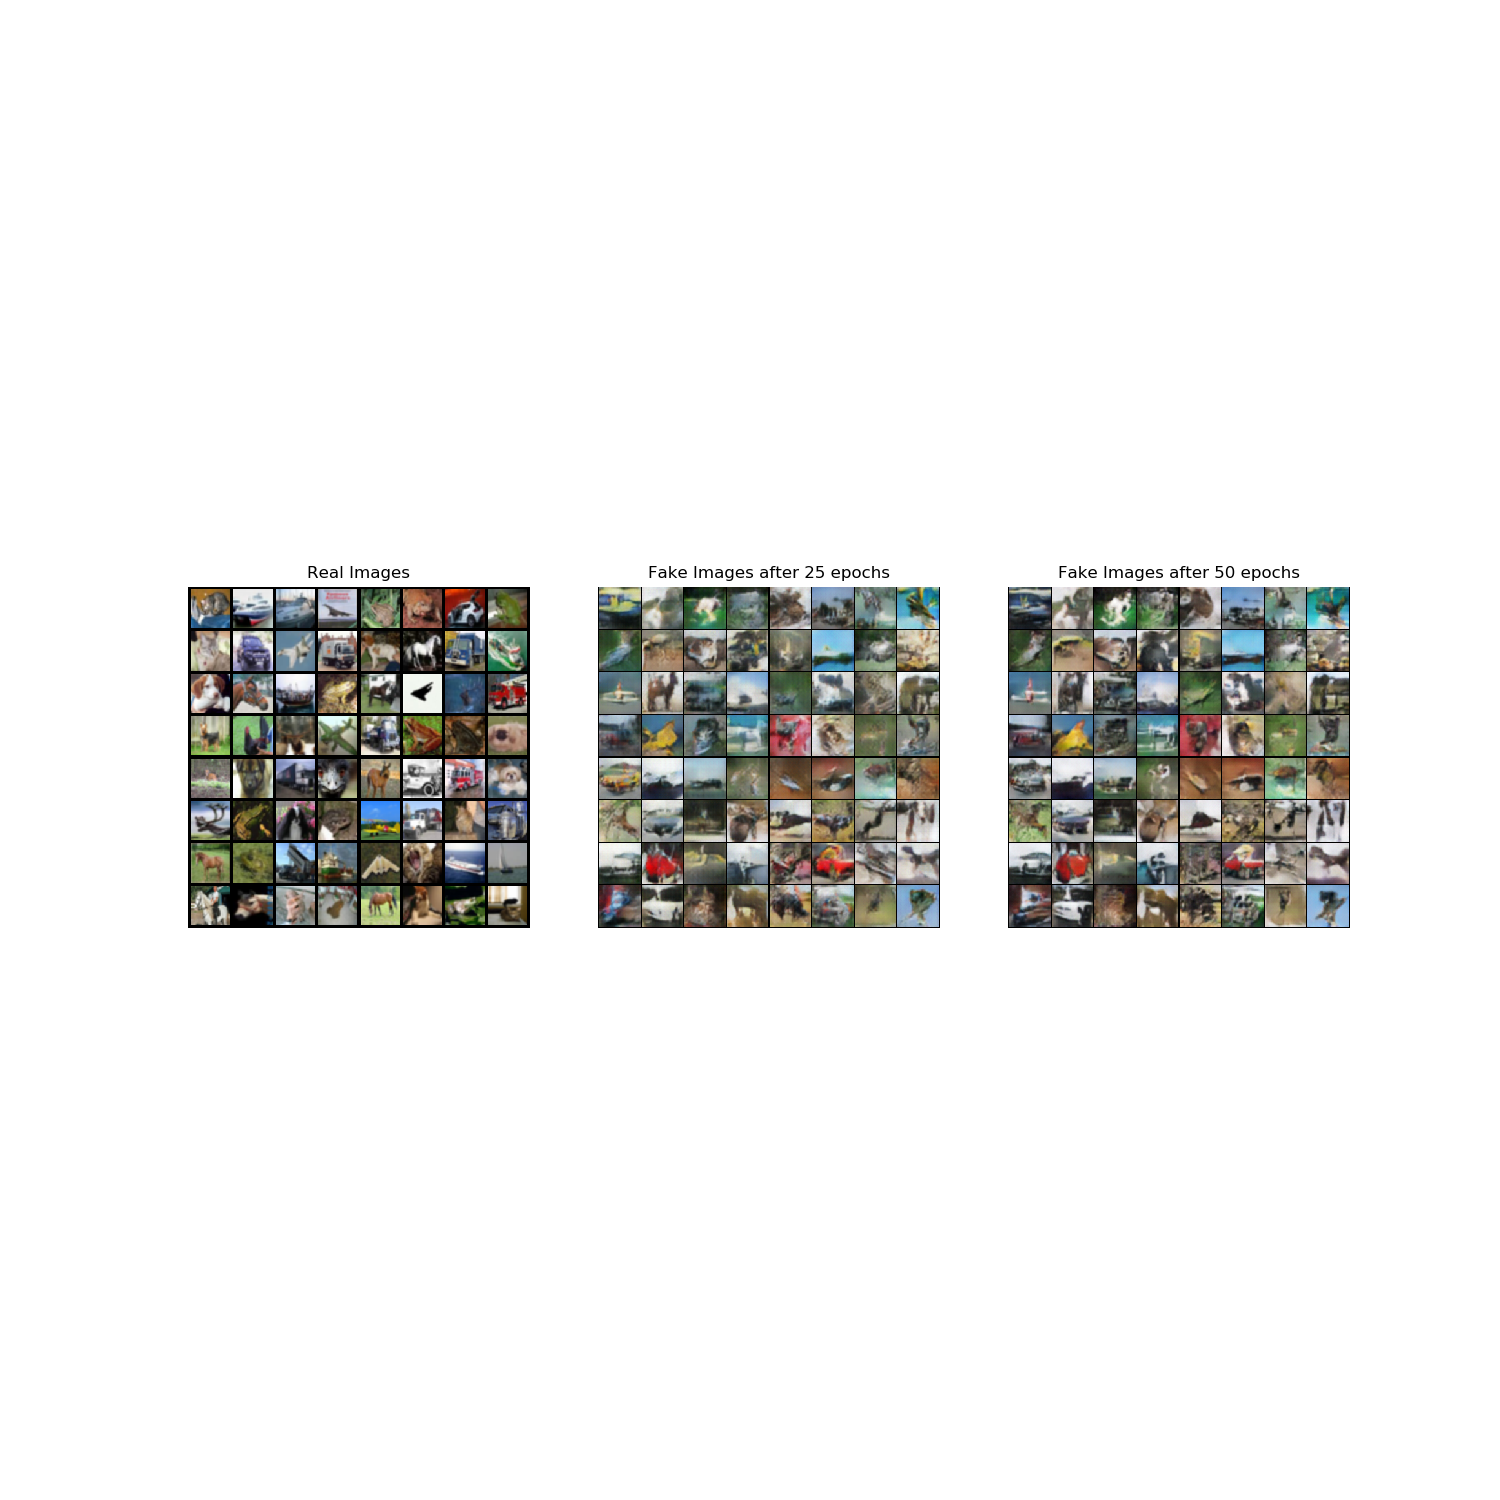
\includegraphics[width=0.75\textwidth]{cifar10_gan_real_v_fake_50_epochs}
\end{figure}

With both datasets, the quality of images does seem to improve with longer training. However, even after 50 epochs the CIFAR10 generated 
images are of disappointing quality. 


\section{Wasserstein GAN Variant}

\begin{figure}[h]
\caption{WGAN Generated MNIST Images After 50 Epochs}
\centering
\includegraphics[width=0.75\textwidth]{MNIST_wgan_real_v_fake_50_epochs}
\end{figure}

\begin{figure}[h]
\caption{WGAN Generated CIFAR10 Images After 50 Epochs}
\centering
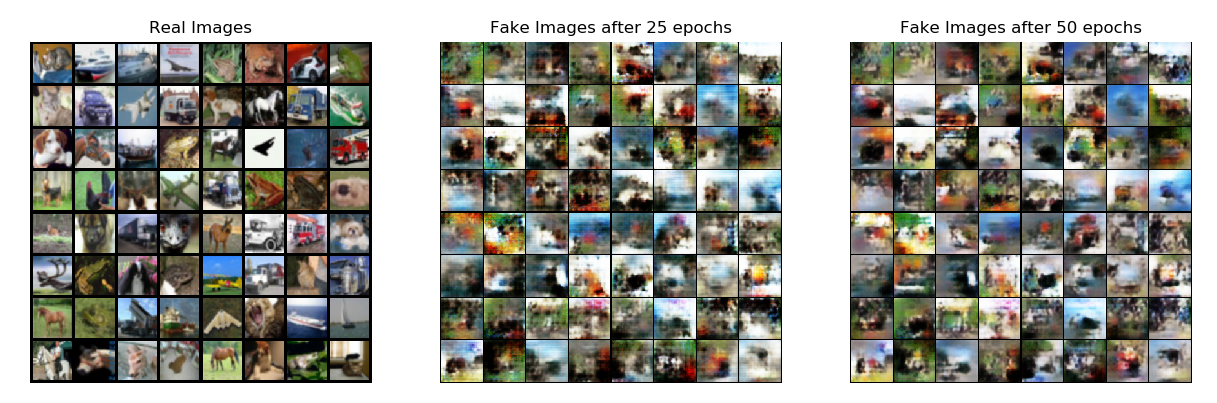
\includegraphics[width=0.75\textwidth]{cifar10_wgan_real_v_fake_50_epochs}
\end{figure}


\section{Conclusion}

\newpage
\bibliographystyle{IEEEtran}
\bibliography{references}

\end{document}
